% Header: Here are all packages used and some additional definitions
%%%%%%%%%%%%%%%%%%%%%%%%%%%%%%%%%%%%%%%%%%%%%%%%%%%%%%%%%%%%%%%%%%%

\documentclass[11pt,a4paper]{scrartcl}
\usepackage[margin=2.5cm]{geometry}
\usepackage[onehalfspacing]{setspace}
\usepackage{graphicx} % zum Einbinden von Graphiken
\usepackage{enumitem}
\usepackage{tcolorbox}
\tcbuselibrary{breakable}
\usepackage[breaklinks=true,colorlinks=true,linkcolor=blue,urlcolor=blue,citecolor=blue]{hyperref} % f. Referenzen
\usepackage{amsmath,amsthm,amssymb} % Mathematik Umgebung 
\usepackage{icomma} % Intelligentes Komma, das den richtigen Abstand zwischen Dezimalzahlen als auch in Formeln wählt.
\usepackage[ngerman]{babel} % Deutsche Bezeichnungen bei Inhaltsangabe etc
\usepackage[T1]{fontenc}    % andere Schriftsatzkodierung für richtige Silbentrennung bei Umlauten
\usepackage[locale = DE,space-before-unit=true,per-mode = symbol]{siunitx} % Bessere Einheiten
\usepackage{booktabs,multirow} % Pakete zur Erstellung von Tabellen
\usepackage{placeins} % Definiert den Befehl “\FloatBarrier”, der die Ausgabe der davor eingebundenen Bilder erzwingt, befor der Text weiter geht. (Mit vorsicht zu verwenden)
\usepackage[natbib,abbreviate=true,doi=false,style=numeric-comp,giveninits=true,sorting=none]{biblatex} % Modernes Paket zur Erzeugung von Bibliografien (benötigt biber!)
\usepackage{csquotes} % Fortgeschrittene Funktionen für Zitate, für die deutsche Form der Anführungszeichen bei Referenzen
%\addbibresource{MyBibliography.bib} % Ort der .bib Datei, die die Datenbank für Literatur/Referenzen enthält.

\graphicspath{{Bilder/} {images/} {chapters/}}

\DeclareSIUnit{\dBm}{dBm}
\DeclareSIUnit[per-mode=reciprocal]\WN{\per\centi\meter}

%%%%%%%%%%%%%%%%%%%%%%%%%%%%%%%%%%%%%%%%%%%%%%%%%%%%%%%%%%%%%%%%%%%
\begin{document}
%
\title{Theoretical Physics 2 - Blatt 02}
\author{Tobias Laser}
\maketitle
\vfill
\thispagestyle{empty}
%
%
\thispagestyle{empty}
\pagenumbering{arabic} 
%
%
\textbf{Aufgabe 1: Delta-Topf Potential (Atom)}: Der Hamiltonoperator eines Teilchens in einer Dimension sei gegeben durch 
\begin{align*}
    H=-\frac{\hbar^2}{2m}\frac{d^2}{dx^2}-\alpha \delta(x),
\end{align*}
mit einer positiven reellen Zahl $\alpha$ (Welche Dimension bzw. Einheit hat $\alpha$?).
\begin{tcolorbox}[title=Berechnung, breakable]
    Da das Argument der Delta-Distribution dimensionslos sein muss, hat $\delta(x)$ die Einheit einer inversen Länge:
    \begin{align*}
        [\delta(x)] &= \frac{1}{[x]} = \frac{1}{\mathrm{m}}
    \end{align*}
    Der Potentialterm $\alpha\delta(x)$ muss die Einheit einer Energie haben. Also gilt
    \begin{align*}
        [E] &= [\alpha \delta(x)] = [\alpha][\delta(x)]\\
        \implies [\alpha] &= \frac{[E]}{[\delta(x)]}
        = [E]\,[x]
        = \frac{\mathrm{kg}\,\mathrm{m}^2}{\mathrm{s}^2}\cdot \mathrm{m}
        = \frac{\mathrm{kg}\,\mathrm{m}^3}{\mathrm{s}^2}
    \end{align*}
    Also hat $\alpha$ die Einheit \emph{Energie} $\times$ \emph{Länge}.
\end{tcolorbox}

\begin{enumerate}[label=(\alph*)]
    \item Integrieren Sie die zugehörige Eigenwertgleichung $H\phi(x) = E \phi(x)$ zwischen den Orten $x_0 = -\epsilon$ und $x_1 = +\epsilon$.
    \begin{tcolorbox}[title=Berechnung, breakable]
        Wir integrieren die Schrödingergleichung über das Intervall $[-\epsilon,+\epsilon]$:
        \begin{align*}
            \int\limits_{-\epsilon}^{+\epsilon}dx\, H \phi(x) &= \int\limits_{-\epsilon}^{+\epsilon} dx\,E \phi(x)
        \end{align*}
        Auf der linken Seite ergibt sich
        \begin{align*}
            \int\limits_{-\epsilon}^{+\epsilon}dx\, H \phi(x)
            &= \int\limits_{-\epsilon}^{+\epsilon}dx\, \left(-\frac{\hbar^2}{2m}\frac{d^2}{dx^2}-\alpha \delta(x)\right) \phi(x)\\
            &= -\frac{\hbar^2}{2m}\int\limits_{-\epsilon}^{+\epsilon}dx\,\phi''(x) -\alpha \int\limits_{-\epsilon}^{+\epsilon}dx\, \delta(x) \phi(x)\\
            &= -\frac{\hbar^2}{2m}\left[ \phi'(x)\right]_{-\epsilon}^{+\epsilon} - \alpha \phi(0)\\
            &= -\frac{\hbar^2}{2m}\left[ \phi'(+\epsilon) - \phi'(-\epsilon)\right] - \alpha \phi(0)
        \end{align*}
        Somit folgt insgesamt
        \begin{align*}
            -\frac{\hbar^2}{2m}\left[\phi'(+\epsilon) - \phi'(-\epsilon)\right] - \alpha \phi(0)
            &= E \int\limits_{-\epsilon}^{+\epsilon} dx\, \phi(x)
        \end{align*}
    \end{tcolorbox}

    Leiten Sie daraus im Limes $\epsilon \rightarrow 0$ ab, dass die Ableitung von $\phi(x)$ einen Sprung bei $x = 0$ besitzt und bestimmen Sie die ``Größe'' der Unstetigkeit als Funktion von $\alpha$, $m$ und $\phi(0)$.
    \begin{tcolorbox}[title=Berechnung, breakable]
        Im Limes $\epsilon \to 0$ verschwindet das Integral auf der rechten Seite,
        \begin{align*}
            \lim\limits_{\epsilon\to0}\int\limits_{-\epsilon}^{+\epsilon} dx\, \phi(x)=0,
        \end{align*}
        sofern $\phi(x)$ bei $x=0$ beschränkt ist. Damit bleibt
        \begin{align*}
            \lim\limits_{\epsilon\to0} \left(-\frac{\hbar^2}{2m}\left[\phi'(+\epsilon) - \phi'(-\epsilon)\right] - \alpha \phi(0)\right) &= 0\\
           -\frac{\hbar^2}{2m}\left[\phi'(0^+) - \phi'(0^-)\right] - \alpha \phi(0) &= 0
        \end{align*}
        und somit
        \begin{align*}
           \phi'(0^+) - \phi'(0^-) &= -\frac{2 m \alpha}{\hbar^2} \phi(0)
        \end{align*}
        Die Ableitung ist also bei $x=0$ unstetig und besitzt dort einen Sprung der Größe
        \begin{align*}
            \Delta \phi' = \phi'(0^+) - \phi'(0^-) = -\frac{2 m \alpha}{\hbar^2} \phi(0).
        \end{align*}
    \end{tcolorbox}

    \item Betrachten Sie den Fall gebundener Zustände, d.h. $E < 0$. Begründen Sie, warum in diesem Fall der allgemeine Ansatz
    \begin{align*}
        \phi(x) = \begin{cases}
            A_1e^{\rho x} + A_1'e^{-\rho x},&x < 0\\
            A_2e^{\rho x} + A_2'e^{-\rho x},& 0 < x
        \end{cases}
    \end{align*}
    gemacht werden kann. Bestimmen Sie $\rho$ als Funktion von $E$, $m$ und $\alpha$. Wie kann $\rho$ physikalisch interpretiert werden?
    \begin{tcolorbox}[title=Berechnung, breakable]
        Für $x\neq 0$ gilt $\delta(x)=0$. Damit reduziert sich die Schrödingergleichung für gebundene Zustände ($E<0$) auf
        \begin{align*}
            -\frac{\hbar^2}{2m}\phi''(x) &= E \phi(x)
        \end{align*}
        Da $E<0$ ist, schreiben wir
        \begin{align*}
            E = -\frac{\hbar^2\rho^2}{2m},
            \qquad \rho>0
        \end{align*}
        Einsetzen liefert
        \begin{align*}
            -\frac{\hbar^2}{2m}\phi''(x) &= -\frac{\hbar^2\rho^2}{2m} \phi(x)\\
            \implies \phi''(x) &= \rho^2\phi(x)
        \end{align*}
        Die allgemeine Lösung dieser Differentialgleichung ist eine Linearkombination von Exponentialfunktionen, also
        \begin{align*}
            \phi(x) = \begin{cases}
                A_1e^{\rho x} + A_1'e^{-\rho x},&x < 0\\
                A_2e^{\rho x} + A_2'e^{-\rho x},& 0 < x
            \end{cases}
        \end{align*}
        Außerdem folgt aus
        \begin{align*}
            E = -\frac{\hbar^2\rho^2}{2m}
        \end{align*}
        direkt
        \begin{align*}
            \rho &= \frac{\sqrt{-2mE}}{\hbar}
        \end{align*}
        also hängt $\rho$ direkt von $E$ und $m$ ab; $\alpha$ geht später über den Rand- bzw. Sprungbedingungen ein.

        Wegen
        \begin{align*}
            [\rho] = \frac{1}{\mathrm{m}}
        \end{align*}
        ist $\rho$ eine inverse Länge. Physikalisch beschreibt $\rho$ also die Abklingrate der Wellenfunktion: Je größer $\rho$ ist, desto stärker ist $\phi(x)$ um $x=0$ lokalisiert.
    \end{tcolorbox}

    \item Zeigen Sie mit (i) der Stetigkeitsbedingung für $\phi(x)$ in $x = 0$, (ii) der Unstetigkeitsbedingung für $\phi'(x)$ aus Teilaufgabe (a) und (iii) der Forderung, dass $\phi(x)$ quadratintegrierbar sein muss, dass nur ein einziger negativer Eigenwert $E$ existiert und bestimmen Sie die zugehörige Eigenfunktion $\phi(x)$. Skizzieren Sie diese Eigenfunktion.
    \begin{tcolorbox}[title=Berechnung, breakable]
        (iii) Aus der Quadratintegrierbarkeit
        \begin{align*}
            \int\limits_{-\infty}^{\infty} dx\, |\phi(x)|^2 < \infty
        \end{align*}
        folgt, dass die Wellenfunktion für $x\to \pm\infty$ nicht divergieren darf. Daher müssen die exponentiell wachsenden Terme verschwinden:
        \begin{align*}
            x\to -\infty \implies e^{-\rho x}\to \infty \implies A_1'=0\\
            x\to +\infty \implies e^{\rho x}\to \infty \implies A_2=0
        \end{align*}
        Somit bleibt
        \begin{align*}
            \phi(x) = \begin{cases}
                A_1e^{\rho x},&x < 0\\
                A_2'e^{-\rho x},&0 < x
            \end{cases}
        \end{align*}

        (i) Wegen der Stetigkeit von $\phi(x)$ bei $x=0$ gilt
        \begin{align*}
            \phi(0^-) &= \phi(0^+)\\
            A_1 &= A_2' =: A
        \end{align*}
        also
        \begin{align*}
            \phi(x) = A e^{-\rho|x|}
            =
            \begin{cases}
                Ae^{\rho x},&x < 0\\
                Ae^{-\rho x},&0 < x
            \end{cases}
        \end{align*}

        (ii) Nun verwenden wir die Sprungbedingung aus Teilaufgabe (a):
        \begin{align*}
            \phi'(0^+) - \phi'(0^-) &= -\frac{2 m \alpha}{\hbar^2} \phi(0)
        \end{align*}
        Mit
        \begin{align*}
            \phi'(0^+) &= - \rho A\\
            \phi'(0^-) &= \rho A\\
            \phi(0) &= A
        \end{align*}
        folgt
        \begin{align*}
            (- \rho A) - (\rho A) &= -\frac{2 m \alpha}{\hbar^2} A\\
            -2\rho A &= -\frac{2 m \alpha}{\hbar^2} A\\
            \implies  \rho &= \frac{m \alpha}{\hbar^2}
        \end{align*}

        Damit ist $\rho$ eindeutig festgelegt, also existiert auch nur ein einziger negativer Eigenwert.

        (Energieeigenwert)
        \begin{align*}
            E &= -\frac{\hbar^2\rho^2}{2m}
            = -\frac{\hbar^2}{2m} \left(\frac{m\alpha}{\hbar^2}\right)^2
            = -\frac{m\alpha^2}{2\hbar^2}
        \end{align*}
        Es existiert daher genau ein gebundener Zustand mit
        \begin{align*}
            E = -\frac{m\alpha^2}{2\hbar^2}
        \end{align*}

        (Aus der Normierungsbedingung)
        \begin{align*}
            \int\limits_{-\infty}^\infty dx\,|\phi(x)|^2 = 1
        \end{align*}
        bestimmen wir nun die Konstante $A$:
        \begin{align*}
            |A|^2 \int\limits_{-\infty}^\infty dx\,e^{-2\rho|x|}
            &= 2|A|^2 \int\limits_0^\infty dx\,e^{-2\rho x}\\
            &= 2 |A|^2 \left[\frac{-1}{2\rho}e^{-2\rho x}\right]_0^\infty\\
            &= 2|A|^2 \frac{1}{2\rho}
            = \frac{|A|^2}{\rho}
        \end{align*}
        also
        \begin{align*}
            A = \sqrt{\rho} = \sqrt{\frac{m\alpha}{\hbar^2}}
        \end{align*}
        wobei wir ohne Beschränkung der Allgemeinheit die positive Wurzel wählen können.

        Damit lautet die normierte Eigenfunktion
        \begin{align*}
            \phi(x) = \sqrt{\frac{m\alpha}{\hbar^2}} \, e^{-\frac{m \alpha}{\hbar^2}|x|}
        \end{align*}

        Die Eigenfunktion ist also gerade, besitzt ihr Maximum bei $x=0$, fällt für $x\to\pm\infty$ exponentiell ab und hat bei $x=0$ einen Knick, d.h. eine unstetige Ableitung.

        Plot

        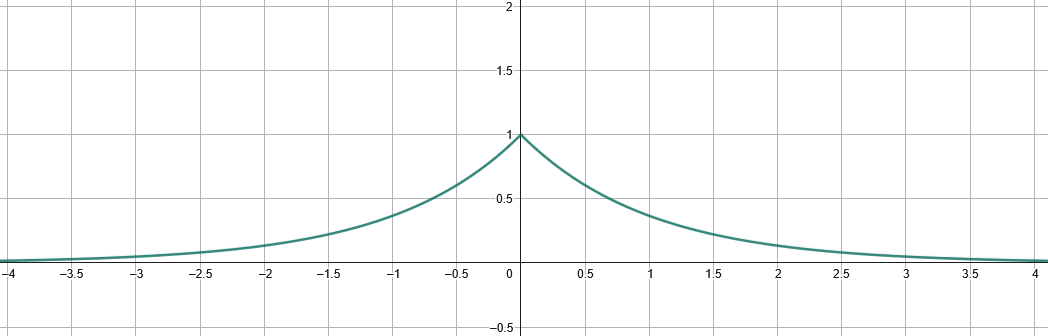
\includegraphics[width=1\textwidth]{Plot.png}
    \end{tcolorbox}

    \item Berechnen Sie die zugehörige Impulsverteilung und die Impulsunschärfe $\Delta p$. Schätzen Sie das Produkt $\Delta x \Delta p$ ab und interpretieren Sie das Ergebnis.
    \begin{tcolorbox}[title=Berechnung, breakable]
        Mit der Fouriertransformierten
        \begin{align*}
            \tilde{\phi}(p) = \frac{1}{\sqrt{2\pi\hbar}} \int\limits_{-\infty}^{\infty} dx\, e^{-ipx/\hbar}\phi(x)
        \end{align*}
        und
        \begin{align*}
            \phi(x) = \sqrt{\rho}\,e^{-\rho |x|}
        \end{align*}
        folgt
        \begin{align*}
            \tilde{\phi}(p) &= \frac{\sqrt{\rho}}{\sqrt{2\pi\hbar}} \int\limits_{-\infty}^{\infty} dx\, e^{-ipx/\hbar} e^{-\rho |x|}\\
            &= \frac{\sqrt{\rho}}{\sqrt{2\pi\hbar}} \left(\int\limits_{-\infty}^{0} dx\, e^{(\rho-ip/\hbar)x} + \int\limits_{0}^{\infty} dx\, e^{-(\rho+ip/\hbar)x}\right)\\
            &= \frac{\sqrt{\rho}}{\sqrt{2\pi\hbar}} \left(\frac{1}{\rho-ip/\hbar} + \frac{1}{\rho+ip/\hbar}\right)\\
            &= \frac{\sqrt{\rho}}{\sqrt{2\pi\hbar}} \frac{2\rho}{\rho^2+(p/\hbar)^2}
        \end{align*}
        also
        \begin{align*}
            \tilde{\phi}(p) = \sqrt{\frac{2\rho}{\pi\hbar}}\,\frac{\rho}{\rho^2+(p/\hbar)^2}
        \end{align*}

        Die Impulsverteilung ist damit
        \begin{align*}
            |\tilde{\phi}(p)|^2 &= \frac{2\rho}{\pi\hbar}\frac{\rho^2}{\left(\rho^2+(p/\hbar)^2\right)^2}\\
            &= \frac{2\rho^3\hbar^3}{\pi\left(p^2+\rho^2\hbar^2\right)^2}
        \end{align*}

        Wegen der Symmetrie von $|\tilde{\phi}(p)|^2$ gilt
        \begin{align*}
            \langle p \rangle = 0
        \end{align*}
        also
        \begin{align*}
            (\Delta p)^2 = \langle p^2\rangle
        \end{align*}

        Für diesen Zustand ergibt sich
        \begin{align*}
            \langle p^2\rangle = \hbar^2\rho^2
        \end{align*}
        und damit
        \begin{align*}
            \Delta p = \hbar\rho
        \end{align*}
        Mit
        \begin{align*}
            \rho = \frac{m\alpha}{\hbar^2}
        \end{align*}
        folgt also
        \begin{align*}
            \Delta p = \hbar \frac{m\alpha}{\hbar^2} = \frac{m\alpha}{\hbar}
        \end{align*}

        Für das Produkt $\Delta x \Delta p$ benötigen wir noch $\Delta x$. Wegen der Symmetrie von $\phi(x)$ gilt
        \begin{align*}
            \langle x \rangle = 0
        \end{align*}
        und
        \begin{align*}
            \langle x^2\rangle &= \int\limits_{-\infty}^{\infty} dx\, x^2 |\phi(x)|^2\\
            &= \rho \int\limits_{-\infty}^{\infty} dx\, x^2 e^{-2\rho |x|}\\
            &= 2\rho \int\limits_{0}^{\infty} dx\, x^2 e^{-2\rho x}\\
            &= 2\rho \frac{2}{(2\rho)^3}\\
            &= \frac{1}{2\rho^2}
        \end{align*}
        daher
        \begin{align*}
            \Delta x = \sqrt{\langle x^2\rangle} = \frac{1}{\sqrt{2}\rho}
        \end{align*}

        Damit folgt
        \begin{align*}
            \Delta x \Delta p = \frac{1}{\sqrt{2}\rho}\cdot \hbar\rho = \frac{\hbar}{\sqrt{2}}
        \end{align*}

        Also gilt
        \begin{align*}
            \Delta x \Delta p = \frac{\hbar}{\sqrt{2}} > \frac{\hbar}{2}
        \end{align*}
        und die Heisenbergsche Unschärferelation ist erfüllt. Das Produkt liegt in der Größenordnung von $\hbar$, aber das Minimum $\hbar/2$ wird nicht erreicht, da $\phi(x)$ keine Gaußfunktion ist.
    \end{tcolorbox}
\end{enumerate}
\newpage
\textbf{Aufgabe 2: Kommutatorrelationen}

Gegeben seien die folgenden Operatoren:
\begin{align*}
    &\text{Ortsoperator:}&(X_j\phi)(\vec{x}) = x_j\phi(\vec{x}),\\ 
    &\text{Impulsoperator:}&(P_j\phi)(\vec{x}) = \frac{\hbar}{i}\frac{\partial}{\partial x_j}\phi(\vec{x}),\\ 
    &\text{Drehimpulsoperator:}&L_j = \sum\limits_{k,l=1}^3 \epsilon_{jkl} X_k P_l,\\ 
    &\text{Gesamtdrehimpuls:}&L^2 = \sum\limits_{k=1}^3 L_k^2,\\ 
    &\text{Hamiltonoperator:}&H = \sum\limits_{k=1}^3 P_k^2/2m + V(r),\\ 
\end{align*}
wobei $j = 1,2,3$ und $r = \sqrt{X_1^2 + X_2^2 + X_3^2}$.

\begin{enumerate}[label=(\alph*)]
    \item Berechnen Sie die Kommutatoren: $[X_j, P_k]$ und $[H, X_j]$, und verwenden Sie dafür Indexschreibweise! Berechnen Sie weiterhin die Kommutatoren $[X_j, (P_j)^n]$ und $[P_j, (X_j)^n]$, und zeigen Sie die Gleichungen
    \begin{align*}
        [X_j, G(P_j)] = i\hbar \frac{\partial G}{\partial P_j},
        \qquad
        [P_j, F(X_j)] = -i\hbar \frac{\partial F}{\partial X_j},
    \end{align*}
    für allgemeine Funktionen $F,G$, die als Potenzreihe geschrieben werden können.
    \begin{tcolorbox}[title=Berechnung, breakable]
        Zunächst berechnen wir $[X_j,P_k]$ durch Wirkung auf eine Testfunktion $\psi(\vec{x})$:
        \begin{align*}
            [X_j,P_k]\psi(\vec{x}) &= X_j(P_k\psi)(\vec{x}) - P_k(X_j\psi)(\vec{x})\\
            &= x_j \frac{\hbar}{i}\frac{\partial}{\partial x_k}\psi(\vec{x}) - \frac{\hbar}{i}\frac{\partial}{\partial x_k}\left(x_j\psi(\vec{x})\right)\\
            &= \frac{\hbar}{i}x_j\frac{\partial}{\partial x_k}\psi(\vec{x}) - \frac{\hbar}{i}\left(\delta_{jk}\psi(\vec{x}) + x_j\frac{\partial}{\partial x_k}\psi(\vec{x})\right)\\
            &= -\frac{\hbar}{i}\delta_{jk}\psi(\vec{x})\\
            &= i\hbar \delta_{jk}\psi(\vec{x})
        \end{align*}
        also
        \begin{align*}
            [X_j,P_k] = i\hbar \delta_{jk}
        \end{align*}

        Weiter gilt
        \begin{align*}
            [H,X_j] &= \left[\sum\limits_{k=1}^3 \frac{P_k^2}{2m} + V(r), X_j\right]\\
            &= \sum\limits_{k=1}^3 \frac{1}{2m}[P_k^2,X_j] + [V(r),X_j]
        \end{align*}
        Da $V(r)$ nur von den Ortsoperatoren abhängt, folgt
        \begin{align*}
            [V(r),X_j] = 0
        \end{align*}
        und mit
        \begin{align*}
            [P_k^2,X_j] &= P_k[P_k,X_j] + [P_k,X_j]P_k\\
            &= P_k(-i\hbar\delta_{jk}) + (-i\hbar\delta_{jk})P_k\\
            &= -2i\hbar\delta_{jk}P_k
        \end{align*}
        erhält man
        \begin{align*}
            [H,X_j] &= \sum\limits_{k=1}^3 \frac{1}{2m}(-2i\hbar\delta_{jk}P_k)\\
            &= -\frac{i\hbar}{m}P_j
        \end{align*}
        also
        \begin{align*}
            [H,X_j] = -\frac{i\hbar}{m}P_j
        \end{align*}

        Nun berechnen wir $[X_j,(P_j)^n]$ induktiv:
        \begin{align*}
            [X_j,(P_j)^n] &= [X_j,P_j(P_j)^{n-1}]\\
            &= [X_j,P_j](P_j)^{n-1} + P_j[X_j,(P_j)^{n-1}]
        \end{align*}
        Für $n=1$ gilt
        \begin{align*}
            [X_j,P_j] = i\hbar
        \end{align*}
        und mit vollständiger Induktion folgt
        \begin{align*}
            [X_j,(P_j)^n] = n\,i\hbar\,(P_j)^{n-1}
        \end{align*}

        Analog:
        \begin{align*}
            [P_j,(X_j)^n] &= [P_j,X_j(X_j)^{n-1}]\\
            &= [P_j,X_j](X_j)^{n-1} + X_j[P_j,(X_j)^{n-1}]\\
            &= -i\hbar (X_j)^{n-1} + X_j[P_j,(X_j)^{n-1}]
        \end{align*}
        also induktiv
        \begin{align*}
            [P_j,(X_j)^n] = -n\,i\hbar\,(X_j)^{n-1}
        \end{align*}

        Sei nun
        \begin{align*}
            G(P_j) = \sum\limits_{n=0}^{\infty} a_n (P_j)^n
        \end{align*}
        eine Potenzreihe. Dann gilt wegen der Linearität des Kommutators
        \begin{align*}
            [X_j,G(P_j)] &= \sum\limits_{n=0}^{\infty} a_n [X_j,(P_j)^n]\\
            &= \sum\limits_{n=1}^{\infty} a_n n\,i\hbar\,(P_j)^{n-1}\\
            &= i\hbar \frac{\partial G}{\partial P_j}
        \end{align*}

        Ebenso für
        \begin{align*}
            F(X_j) = \sum\limits_{n=0}^{\infty} b_n (X_j)^n
        \end{align*}
        folgt
        \begin{align*}
            [P_j,F(X_j)] &= \sum\limits_{n=0}^{\infty} b_n [P_j,(X_j)^n]\\
            &= \sum\limits_{n=1}^{\infty} b_n (-n\,i\hbar)(X_j)^{n-1}\\
            &= -i\hbar \frac{\partial F}{\partial X_j}
        \end{align*}

        Insgesamt also
        \begin{align*}
            [X_j,P_k] &= i\hbar \delta_{jk}\\
            [H,X_j] &= -\frac{i\hbar}{m}P_j\\
            [X_j,(P_j)^n] &= n\,i\hbar\,(P_j)^{n-1}\\
            [P_j,(X_j)^n] &= -n\,i\hbar\,(X_j)^{n-1}\\
            [X_j,G(P_j)] &= i\hbar \frac{\partial G}{\partial P_j}\\
            [P_j,F(X_j)] &= -i\hbar \frac{\partial F}{\partial X_j}
        \end{align*}
    \end{tcolorbox}

    \item Berechnen Sie die Kommutatoren: $[L_j,X_k]$, $[L_j,P_k]$ und $[L_j,L_k]$, und $[L^2,L_j]$.
    \begin{tcolorbox}[title=Berechnung, breakable]
        Mit
        \begin{align*}
            L_j = \sum\limits_{m,n=1}^3 \epsilon_{jmn}X_mP_n
        \end{align*}
        gilt
        \begin{align*}
            [L_j,X_k] &= \sum\limits_{m,n=1}^3 \epsilon_{jmn}[X_mP_n,X_k]\\
            &= \sum\limits_{m,n=1}^3 \epsilon_{jmn}\left(X_m[P_n,X_k] + [X_m,X_k]P_n\right)
        \end{align*}
        Wegen $[X_m,X_k]=0$ und
        \begin{align*}
            [P_n,X_k] = -i\hbar \delta_{nk}
        \end{align*}
        folgt
        \begin{align*}
            [L_j,X_k] &= \sum\limits_{m,n=1}^3 \epsilon_{jmn}X_m(-i\hbar\delta_{nk})\\
            &= -i\hbar \sum\limits_{m=1}^3 \epsilon_{jmk}X_m
        \end{align*}
        Umgeschrieben ergibt das die Standardform
        \begin{align*}
            [L_j,X_k] = i\hbar \sum\limits_{m=1}^3 \epsilon_{jkm}X_m
        \end{align*}

        Analog:
        \begin{align*}
            [L_j,P_k] &= \sum\limits_{m,n=1}^3 \epsilon_{jmn}[X_mP_n,P_k]\\
            &= \sum\limits_{m,n=1}^3 \epsilon_{jmn}\left(X_m[P_n,P_k] + [X_m,P_k]P_n\right)
        \end{align*}
        Da $[P_n,P_k]=0$ und
        \begin{align*}
            [X_m,P_k] = i\hbar \delta_{mk}
        \end{align*}
        folgt
        \begin{align*}
            [L_j,P_k] &= \sum\limits_{m,n=1}^3 \epsilon_{jmn}(i\hbar\delta_{mk})P_n\\
            &= i\hbar \sum\limits_{n=1}^3 \epsilon_{jkn}P_n
        \end{align*}
        also
        \begin{align*}
            [L_j,P_k] = i\hbar \sum\limits_{m=1}^3 \epsilon_{jkm}P_m
        \end{align*}

        Für $[L_j,L_k]$ verwenden wir das Resultat aus den beiden vorherigen Rechnungen:
        \begin{align*}
            [L_j,L_k] &= \left[L_j,\sum\limits_{m,n=1}^3 \epsilon_{kmn}X_mP_n\right]\\
            &= \sum\limits_{m,n=1}^3 \epsilon_{kmn}[L_j,X_mP_n]\\
            &= \sum\limits_{m,n=1}^3 \epsilon_{kmn}\left([L_j,X_m]P_n + X_m[L_j,P_n]\right)
        \end{align*}
        Einsetzen von
        \begin{align*}
            [L_j,X_m] &= i\hbar \sum\limits_{a=1}^3 \epsilon_{jma}X_a\\
            [L_j,P_n] &= i\hbar \sum\limits_{b=1}^3 \epsilon_{jnb}P_b
        \end{align*}
        liefert
        \begin{align*}
            [L_j,L_k]
            &= i\hbar \sum\limits_{m,n,a=1}^3 \epsilon_{kmn}\epsilon_{jma}X_aP_n
            + i\hbar \sum\limits_{m,n,b=1}^3 \epsilon_{kmn}\epsilon_{jnb}X_mP_b
        \end{align*}
        Nach Auswertung der Levi-Civita-Kontraktionen erhält man
        \begin{align*}
            [L_j,L_k] = i\hbar \sum\limits_{m=1}^3 \epsilon_{jkm}L_m
        \end{align*}

        Nun zu $[L^2,L_j]$:
        \begin{align*}
            [L^2,L_j] &= \left[\sum\limits_{k=1}^3 L_k^2,L_j\right]\\
            &= \sum\limits_{k=1}^3 [L_k^2,L_j]\\
            &= \sum\limits_{k=1}^3 \left(L_k[L_k,L_j] + [L_k,L_j]L_k\right)
        \end{align*}
        Mit
        \begin{align*}
            [L_k,L_j] = i\hbar \sum\limits_{m=1}^3 \epsilon_{kjm}L_m
        \end{align*}
        folgt
        \begin{align*}
            [L^2,L_j]
            &= i\hbar \sum\limits_{k,m=1}^3 \epsilon_{kjm}(L_kL_m + L_mL_k)
        \end{align*}
        Da $L_kL_m + L_mL_k$ symmetrisch in $k,m$ ist, $\epsilon_{kjm}$ aber antisymmetrisch, verschwindet die Summe:
        \begin{align*}
            [L^2,L_j] = 0
        \end{align*}

        Insgesamt:
        \begin{align*}
            [L_j,X_k] &= i\hbar \sum\limits_{m=1}^3 \epsilon_{jkm}X_m\\
            [L_j,P_k] &= i\hbar \sum\limits_{m=1}^3 \epsilon_{jkm}P_m\\
            [L_j,L_k] &= i\hbar \sum\limits_{m=1}^3 \epsilon_{jkm}L_m\\
            [L^2,L_j] &= 0
        \end{align*}
    \end{tcolorbox}

    \item Berechnen Sie die Kommutatoren: $[H,P_j]$, $[H,L_j]$ und $[H,L^2]$.
    \begin{tcolorbox}[title=Berechnung, breakable]
        Zunächst:
        \begin{align*}
            [H,P_j] &= \left[\sum\limits_{k=1}^3 \frac{P_k^2}{2m} + V(r),P_j\right]\\
            &= \sum\limits_{k=1}^3 \frac{1}{2m}[P_k^2,P_j] + [V(r),P_j]
        \end{align*}
        Da die Impulsoperatoren paarweise kommutieren, gilt
        \begin{align*}
            [P_k^2,P_j] = 0
        \end{align*}
        also
        \begin{align*}
            [H,P_j] = [V(r),P_j]
        \end{align*}
        Aus Teil (a) wissen wir bereits
        \begin{align*}
            [P_j,F(X_j)] = -i\hbar \frac{\partial F}{\partial X_j}
        \end{align*}
        also äquivalent
        \begin{align*}
            [F(X_1,X_2,X_3),P_j] = i\hbar \frac{\partial F}{\partial X_j}
        \end{align*}
        Damit folgt
        \begin{align*}
            [V(r),P_j] = i\hbar \frac{\partial V(r)}{\partial X_j}
        \end{align*}
        Wegen der Kettenregel
        \begin{align*}
            \frac{\partial V(r)}{\partial X_j} = \frac{dV}{dr}\frac{\partial r}{\partial X_j}
        \end{align*}
        und
        \begin{align*}
            r = \sqrt{X_1^2+X_2^2+X_3^2}
            \implies
            \frac{\partial r}{\partial X_j} = \frac{X_j}{r}
        \end{align*}
        also
        \begin{align*}
            [H,P_j] = i\hbar \frac{dV}{dr}\frac{X_j}{r}
        \end{align*}

        Nun:
        \begin{align*}
            [H,L_j] &= \left[\sum\limits_{k=1}^3 \frac{P_k^2}{2m} + V(r),L_j\right]\\
            &= \sum\limits_{k=1}^3 \frac{1}{2m}[P_k^2,L_j] + [V(r),L_j]
        \end{align*}

        Für den kinetischen Term:
        \begin{align*}
            [P_k^2,L_j] &= P_k[P_k,L_j] + [P_k,L_j]P_k
        \end{align*}
        mit
        \begin{align*}
            [P_k,L_j] = -[L_j,P_k] = -i\hbar \sum\limits_{m=1}^3 \epsilon_{jkm}P_m
        \end{align*}
        also
        \begin{align*}
            [P_k^2,L_j]
            &= -i\hbar \sum\limits_{m=1}^3 \epsilon_{jkm}(P_kP_m + P_mP_k)
        \end{align*}
        Da $P_kP_m + P_mP_k$ symmetrisch in $k,m$ ist und $\epsilon_{jkm}$ antisymmetrisch, folgt
        \begin{align*}
            \sum\limits_{k=1}^3 \frac{1}{2m}[P_k^2,L_j] = 0
        \end{align*}

        Für den Potentialterm:
        \begin{align*}
            [V(r),L_j]
            &= \left[V(r),\sum\limits_{k,\ell=1}^3 \epsilon_{jk\ell}X_kP_\ell\right]\\
            &= \sum\limits_{k,\ell=1}^3 \epsilon_{jk\ell}[V(r),X_kP_\ell]\\
            &= \sum\limits_{k,\ell=1}^3 \epsilon_{jk\ell}\left([V(r),X_k]P_\ell + X_k[V(r),P_\ell]\right)
        \end{align*}
        Da $V(r)$ nur von den Ortsoperatoren abhängt, gilt
        \begin{align*}
            [V(r),X_k] = 0
        \end{align*}
        und somit
        \begin{align*}
            [V(r),L_j]
            &= \sum\limits_{k,\ell=1}^3 \epsilon_{jk\ell}X_k \left(i\hbar \frac{dV}{dr}\frac{X_\ell}{r}\right)\\
            &= i\hbar \frac{dV}{dr}\frac{1}{r}\sum\limits_{k,\ell=1}^3 \epsilon_{jk\ell}X_kX_\ell
        \end{align*}
        Da $X_kX_\ell$ symmetrisch in $k,\ell$ ist und $\epsilon_{jk\ell}$ antisymmetrisch, verschwindet auch diese Summe:
        \begin{align*}
            [V(r),L_j] = 0
        \end{align*}
        also insgesamt
        \begin{align*}
            [H,L_j] = 0
        \end{align*}

        Schließlich:
        \begin{align*}
            [H,L^2] &= \left[H,\sum\limits_{j=1}^3 L_j^2\right]\\
            &= \sum\limits_{j=1}^3 [H,L_j^2]\\
            &= \sum\limits_{j=1}^3 \left([H,L_j]L_j + L_j[H,L_j]\right)
        \end{align*}
        Wegen $[H,L_j]=0$ folgt
        \begin{align*}
            [H,L^2] = 0
        \end{align*}

        Insgesamt:
        \begin{align*}
            [H,P_j] &= i\hbar \frac{dV}{dr}\frac{X_j}{r}\\
            [H,L_j] &= 0\\
            [H,L^2] &= 0
        \end{align*}
    \end{tcolorbox}
\end{enumerate}


\end{document}
